\documentclass{article}
\usepackage[utf8]{inputenc}
\usepackage[left=2cm,right=2cm,top=2cm,bottom=2cm]{geometry}
\usepackage{amsthm, amsmath, mathtools, amssymb}
\usepackage[sorting=none]{biblatex}
\usepackage{booktabs}
\usepackage{caption}
\usepackage{subcaption}
\usepackage{algpseudocode}
\usepackage{algorithm}

\floatname{algorithm}{}
\renewcommand{\algorithmicrequire}{\textbf{ENTRADA: }}
\renewcommand{\algorithmicensure}{\textbf{SORTIDA: }}

\addbibresource{references.bib}


\newcommand{\rvline}{\hspace*{-\arraycolsep}\vline\hspace*{-\arraycolsep}}
  
\makeatother
\newtheorem{definition}{Definició}[section]
\newtheorem{example}{Exemple}[section]
\newtheorem{theorem}{Teorema}[section]
\newtheorem{corollary}{Corol·lari}[section]
\newtheorem{lemma}{Lema}[section]
\newtheorem{prop}{Proposició}[section]
\renewcommand*{\proofname}{Demostració}

\renewcommand*\contentsname{Índex}
\renewcommand*\figurename{Figura}
\renewcommand*\tablename{Taula}

\emergencystretch=3em

\begin{document}

\begin{titlepage}
\begin{center}
\vspace*{0in}
\begin{figure}[H]
    \begin{center}
    
\includegraphics[width=6cm]{imatges/uab.jpg}
    \end{center}
\end{figure}
\rule{130mm}{0.1mm}\\
\Large{\textbf{UNIVERSITAT AUTÒNOMA DE BARCELONA}} \\
\vspace*{0.5in}
\begin{large}
SEMINARI DE MATEMÀTICA DISCRETA \\
\end{large}
\vspace*{1in}
\begin{LARGE}
\textbf{ARBRE GENERADOR MINIMAL. QUANTS ARBRES GENERADORS ADMET UN GRAF?} \\
\end{LARGE}
\vspace*{1in}
\begin{abstract}
    En aquest treball ens centrem principalment en l'estudi del nombre d'arbres generadors d'un graf. Primer de tot, començarem enunciant una fórmula del cas particular en què el graf és un graf complet i a continuació ge\-ne\-ra\-lit\-za\-rem el concepte per a grafs arbitraris. Finalment, introduirem els arbres generadors ponderats, exposarem aplicacions d'aquest tema i descriurem mètodes computacionals per trobar l'arbre generador ponderat minimal d'un graf. 
\end{abstract}
\vspace*{1.3in}
\begin{large}
Presentat per:\\
\vspace*{0.1in}
Víctor Ballester Ribó \\
Oriol Bosquet Gallardo\\
Eric Recio Chorro\\
Carlo Sala Gancho\\
\end{large}
\vspace*{0.2in}
\rule{80mm}{0.1mm}\\
\vspace*{0.1in}
\begin{large}
Gener de 2021
\end{large}
\end{center}
\newpage
\end{titlepage}
\newpage
\tableofcontents
\newpage

\section{Definicions prèvies}
    Comencem aquest treball definint els conceptes necessaris en relació amb els grafs i, en particular, amb els arbres.
    \begin{definition}[Graf]
        Un graf $G$ consisteix en una parella $(V(G), E(G))$ on:
        \begin{itemize}
            \item $V(G)$ és un conjunt (no buit) d'elements, anomenats vèrtexs del graf.
            \item $E(G)$ és un multiconjunt de parelles no ordenades de vèrtexs, que anomenem arestes del graf.
        \end{itemize}
    \end{definition}
    \begin{definition}[Graf simple]
        Sigui $G$ un graf. Diem que $G$ és simple si no té cap aresta múltiple (més d'una aresta entre els mateixos vèrtexs) ni bucles (arestes que van d'un vèrtex en ell mateix).
    \end{definition}
    \begin{definition}[Multigraf]
        Diem que $G$ és un multigraf si té, com a mínim, una aresta múltiple o bé un bucle.
    \end{definition}
    Per conveni, quan parlem de grafs ens referirem a grafs simples. Quan vulguem considerar grafs que no siguin simples, ens hi referirem com a multigrafs.
    \begin{definition}
    Un \textit{passeig de longitud} $k$ en un graf $G$ és una successió de vèrtexs $(u_1,\ldots,u_k)$ on $u_iu_{i+1}\in E(G)$ per $i=1,\ldots,k-1$.
    \end{definition}
    \begin{definition}
    Un passeig en un graf és \textit{tancat} si comença i acaba al mateix vèrtex.
    \end{definition}
    \begin{definition}
    Un passeig en un graf és un \textit{camí} si totes les arestes del passeig són diferents.
    \end{definition}
    \begin{definition}
    Un passeig en un graf és un \textit{camí simple} si és un camí i tots els vèrtexs del passeig són diferents.
    \end{definition}
    \begin{definition}
    Un passeig tancat en un graf és un \textit{camí tancat} si totes les arestes del passeig tancat són diferents.
    \end{definition}
    \begin{definition}
    Un camí simple tancat s'anomena \textit{cicle}.
    \end{definition}
    \begin{definition}
    Un graf $G$ és \textit{connex} si $\forall u,v\in V(G)$ hi ha un camí simple a $G$ que va de $u$ a $v$.
    \end{definition}
    \begin{definition}[Arbre]
        Sigui $G$ un graf. Diem que $G$ és un arbre si $G$ és connex i no té cicles.
    \end{definition}
    \begin{definition}[Fulla]
    Sigui $T$ un arbre. Definim una fulla de $T$ com un vèrtex de grau 1.
    \end{definition}
    \begin{definition}[Subgraf generador]
        Sigui $G$ un graf connex. Un subgraf generador $G'$ de $G$ és un subgraf de $G$ tal que $V(G')=V(G)$. En particular, un arbre generador $T$ de $G$ és un subgraf generador de $G$ tal que $T$ és un arbre.
    \end{definition}
    \begin{definition}[Matriu d'incidència]
        Sigui $G$ un graf i sigui $n=|V(G)|$ i $m=|E(G)|$. La matriu d'incidència de $G$ és una matriu $M=(m_{ij})\in\mathcal{M}_{n\times m}(\mathbb{R})$ tal que:
        $$m_{ij}=\left\{\begin{array}{ll}
            1 & \text{si l'aresta $j$ és incident amb el vèrtex $i$,} \\
            0 & \text{altrament.}
        \end{array}\right.$$
    \end{definition}
    Observem que la matriu d'incidència d'un graf tindrà exactament dos 1 en cada columna. Això ens condueix a definir la següent matriu:
    \begin{definition}[Matriu d'incidència orientada]
    Sigui $G$ un graf i $M$ la seva matriu d'incidència. Definim la matriu d'incidència orientada $M'$ de $G$ com la matriu $M$ on a cada columna canviem exactament un $1$ per un $-1$.\footnote{Aquest nom de ``matriu d'incidència orientada" l'hem adoptat així ja que aquesta matriu és precisament la matriu d'incidència d'un graf dirigit o orientat.} \cite{10}
    \end{definition}
    Per no fer un abús de notació, a partir d'ara denotarem per $M$ la matriu d'incidència orientada. Fixem-nos que en aquesta matriu una de les files és supèrflua, ja que coneixent totes les altres i tenint en compte que en cada columna hi ha exactament un 1 i un $-1$, podem deduir què contindrà aquesta fila en qüestió. Això dona lloc a definir la següent matriu:
    \begin{definition}[Matriu d'incidència orientada reduïda]
    Sigui $G$ un graf i $M$ la seva matriu d'incidència orientada. Definim la matriu d'incidència orientada reduïda $M_0$ com la matriu $M$ en la qual s'ha eliminat una fila. El vèrtex corresponent a aquesta fila eliminada l'anomenarem vèrtex de referència. En aquest treball, per conveni, eliminarem sempre la darrera fila. \cite{2}
    \end{definition}
    Per simplificar l'escriptura, d'ara endavant ens referirem a la matriu d'incidència orientada reduïda simplement com a matriu d'incidència reduïda, entenent que és la matriu amb 1's i $-1$'s.
    \begin{definition}
    Sigui $G$ un graf, $M_0$ la seva matriu d'incidència reduïda i $T$ un arbre generador de $G$. Definim la matriu d'incidència reduïda de $T$ com la matriu quadrada $M_0[T]$ obtinguda seleccionant les $n-1$ columnes de $M_0$ corresponents a les arestes de $T$ en $G$. \cite{2}
    \end{definition}
    \begin{definition}[Matriu de Laplace]
        Sigui $G$ un graf i sigui $n=|V(G)|$. Definim la matriu de Laplace $L=(\ell_{ij})\in\mathcal{M}_n(\mathbb{R})$ com:
        $$\ell_{ij}=\left\{\begin{array}{cl}
            \deg v_i & \text{si $i=j$,}\\
            -1 & \text{si els vèrtexs $v_i$ i $v_j$ són adjacents,}\\
            0 & \text{altrament.}
        \end{array}\right.$$\cite{9}
    \end{definition}
    Per clarificar aquestes definicions, posem un exemple on calculem totes les matrius que hem definit:
    \begin{example}\label{exempl1}
        Sigui $G$ el graf de la figura \ref{g1}. Aquest graf té les següents matrius associades:\newline
        Matriu d'incidència:
        $$\Tilde{M}=
        \begin{pmatrix}
            1 & 1 & 1 & 1 & 0 & 0 & 0 \\
            0 & 1 & 0 & 0 & 1 & 0 & 1 \\
            0 & 0 & 0 & 1 & 1 & 0 & 0 \\
            0 & 0 & 1 & 0 & 0 & 1 & 0 \\
            1 & 0 & 0 & 0 & 0 & 1 & 1
        \end{pmatrix}.
        $$
        Matriu d'incidència orientada:
        $$M=
        \begin{pmatrix}
            1 & 1 & 1 & 1 & 0 & 0 & 0 \\
            0 & -1 & 0 & 0 & 1 & 0 & 1 \\
            0 & 0 & 0 & -1 & -1 & 0 & 0 \\
            0 & 0 & -1 & 0 & 0 & 1 & 0 \\
            -1 & 0 & 0 & 0 & 0 & -1 & -1
        \end{pmatrix}.
        $$
        Matriu d'incidència orientada reduïda:
        $$M_0=
        \begin{pmatrix}
            1 & 1 & 1 & 1 & 0 & 0 & 0 \\
            0 & -1 & 0 & 0 & 1 & 0 & 1 \\
            0 & 0 & 0 & -1 & -1 & 0 & 0 \\
            0 & 0 & -1 & 0 & 0 & 1 & 0
        \end{pmatrix}.
        $$
        Matriu de Laplace:
        $$L=
        \begin{pmatrix}
            4 & -1 & -1 & -1 & -1 \\
            -1 & 3 & -1 & 0 & -1 \\
            -1 & -1 & 2 & 0 & 0 \\
            -1 & 0 & 0 & 2 & -1 \\
            -1 & -1 & 0 & -1 & 3
        \end{pmatrix}.
        $$
        A més, si considerem l'arbre generador de la figura \ref{g2}, tenim que la matriu d'incidència reduïda associada a l'arbre $T$ és:
        $$M_0[T]=
        \begin{pmatrix}
            1 & 1 & 0 & 0 \\
            0 & 0 & 0 & 1 \\
            0 & -1 & 0 & 0 \\
            -1 & 0 & 1 & 0
        \end{pmatrix}.
        $$
        Observem que, com veurem més endavant en el lema \ref{1}, tenim aquesta igualtat: $L=MM^t$.
        \begin{figure}[H]
    \centering
    \begin{subfigure}{.45\textwidth}
        \centering
        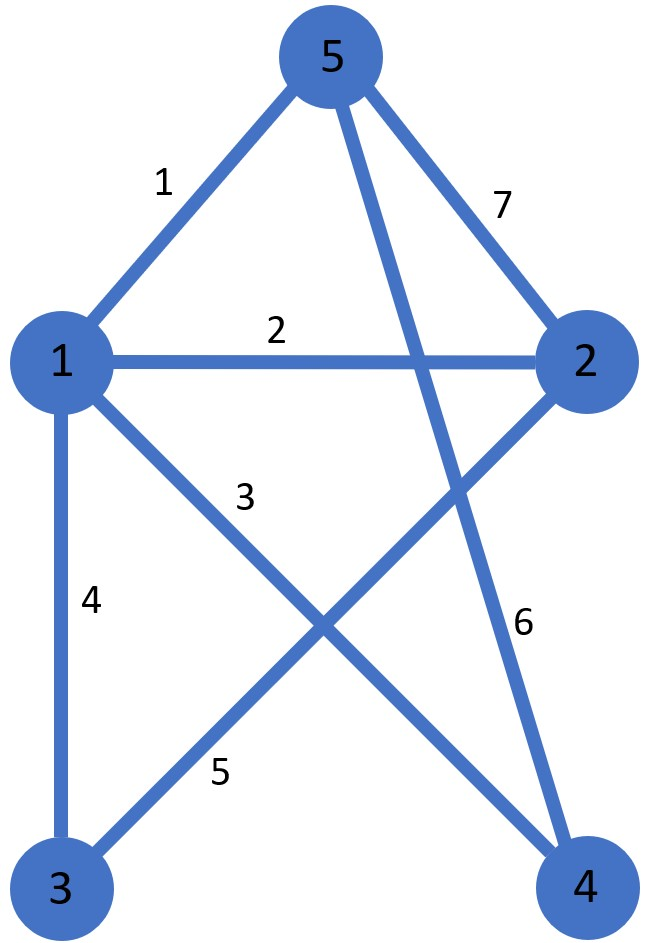
\includegraphics[width=4cm]{imatges/exemple1.jpg}
        \caption{Graf.}
        \label{g1}
    \end{subfigure}
    \begin{subfigure}{.45\textwidth}
        \centering
        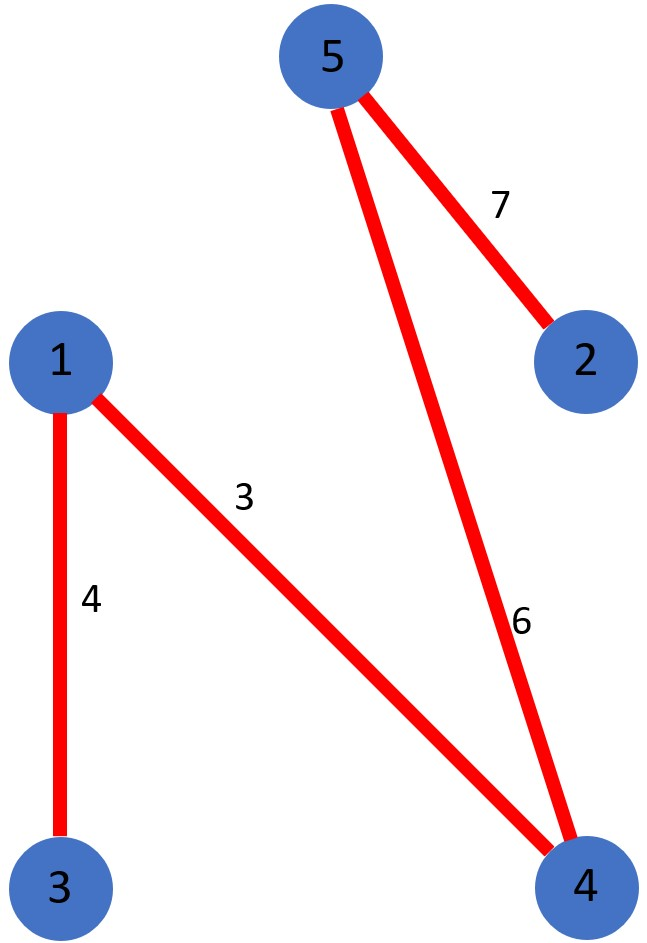
\includegraphics[width=4cm]{imatges/exemple2.jpg}
        \caption{Arbre generador del graf}
        \label{g2}
    \end{subfigure}
    \caption{Graf de l'exemple \ref{exempl1}}
\end{figure}
    \end{example}
\section{Fórmula de Cayley}
El 1889 Arthur Cayley va establir una fórmula per determinar el nombre d'arbres generadors diferents del graf complet $K_n$ amb l'etiquetació dels vèrtexs $[n] = \{1,2,\dots ,n\}$. Hi ha moltes demostracions d'aquesta fórmula. En aquest treball en donarem una, presentada l'any 1918 pel matemàtic alemany Heinz Prüfer, establint una correspondència bijectiva entre arbres generadors amb $n$ vèrtexs i els anomenats codis de Prüfer (successions de longitud $n-2$). \cite{5}\par
Com hem mencionat, per veure la demostració de la fórmula de Cayley primer és necessari definir la seqüència de Prüfer.
\begin{definition}\label{pruf}
Sigui $T$ un arbre d'ordre $n \geq 3$ amb conjunt de vèrtexs $V(T)= [n]$. Definim la seqüència de Prüfer com la successió
$$\mathcal{P}(T)=(y_1,y_2,\ldots,y_{n-2})$$
de $n-2$ nombres del conjunt $V(T)=[n]$. Amb el següent algorisme, podem codificar qualsevol arbre en una seqüència de Prüfer:
\begin{enumerate}
\item Prenem la fulla de l'arbre $T$ amb etiqueta menor. Eliminem aquesta fulla de $T$ i li assignem el valor de l'etiqueta del seu únic vèrtex adjacent.
\item Continuem el procés amb l'arbre creat a partir de $T$ en eliminar la fulla anterior i repetim l'algorisme fins que ens quedi un arbre d'un vèrtex. Haurem obtingut una seqüència de $n-1$ nombres, que, descartant l'últim d'ells es transforma amb una seqüència de $n-2$ termes. \cite{4}
\end{enumerate}
\end{definition}
Notem que aquesta seqüència d'un arbre és única. En efecte, si $T$ és l'arbre considerat en qüestió i $\mathcal{P}(T)$ la seva seqüència de Prüfer, observem primer que les etiquetes de les fulles de $T$ no estan representades en $\mathcal{P}(T)$, ja que una fulla no pot ser adjacent a una altra fulla (considerant arbres d'ordre $n\geq 3$). Per tant, d'aquí es dedueix que cada vèrtex té grau igual a $1+a$, on $a$ és el nombre de vegades que apareix el vèrtex a $\mathcal{P}(T)$. A la figura \ref{pruf1} podem veure un exemple de com trobar la seqüència de Prüfer d'un arbre.\par \begin{figure}[H]
   \centering
   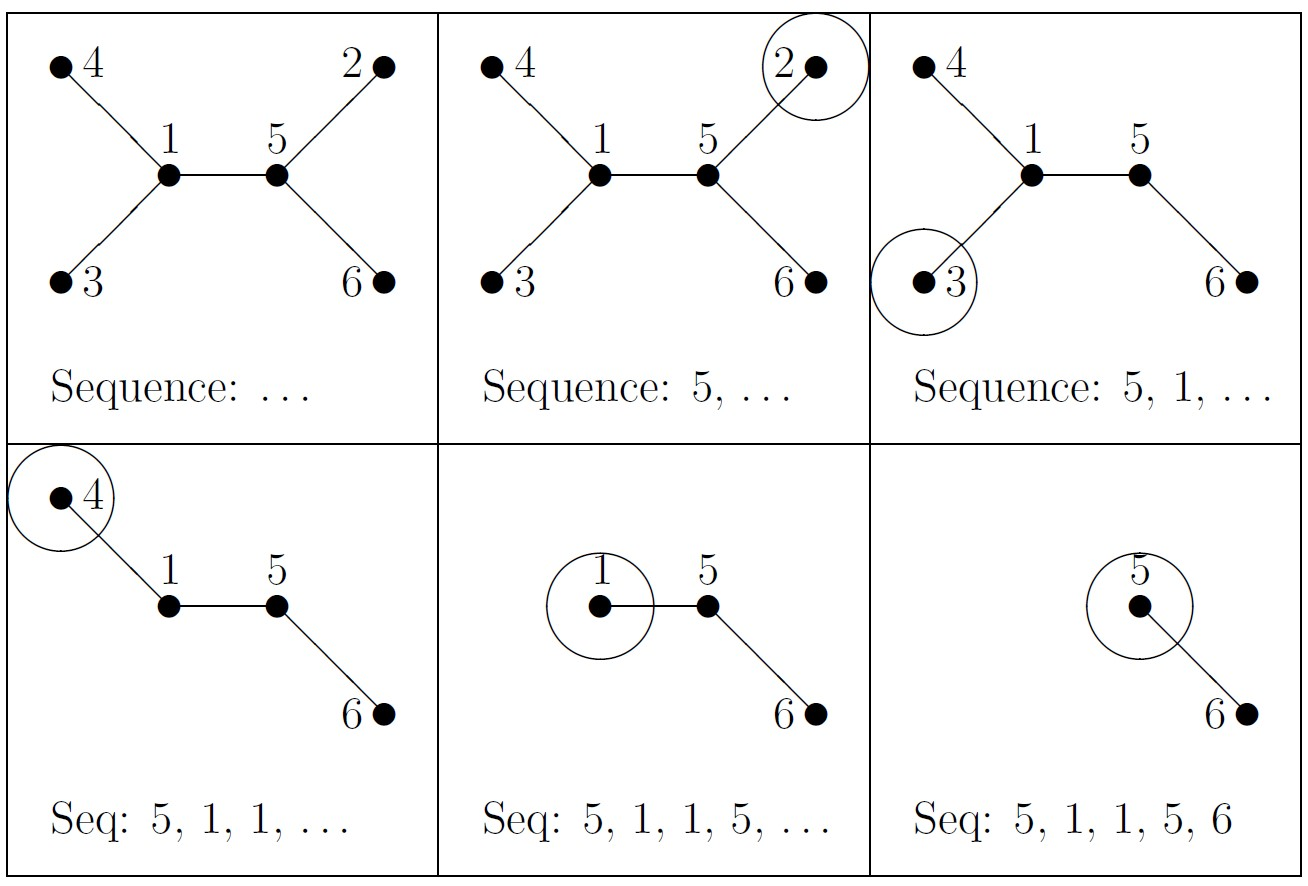
\includegraphics[width=9cm]{imatges/prufer1.jpg}
   \caption{A partir de l'arbre indicat a les imatges, considerem primer la fulla d'índex menor, en aquest cas el vèrtex 2. Afegim doncs a la seqüència de Prüfer l'etiqueta del vèrtex adjacent al vèrtex 2, és a dir, el número 5. A continuació, eliminem l'aresta que uneix els vèrtexs 2 i 5 i repetim el procés. Notem que al final acabem amb una seqüència de 5 nombres. No obstant això, l'últim el podem eliminar. \cite{3}}
   \label{pruf1}
\end{figure}
El següent resultat ens diu que si tenim una seqüència de $n-2$ termes, automàticament també tenim un arbre $T$ amb seqüència de Prüfer igual a la que estàvem considerant.
\begin{prop}
Sigui $\mathcal{P}=(y_1,\ldots,y_{n-2})$ una seqüència de $n-2$ dígits. Aleshores, $\mathcal{P}$ és la seqüència de Prüfer d'un arbre $T$, és a dir, $\mathcal{P}=\mathcal{P}(T)$.
\end{prop}
\begin{proof}
Crearem l'arbre $T$ a partir de $\mathcal{P}$ de la següent manera:
\begin{enumerate}
    \item Trobem el nombre més petit del conjunt $[n]$ que no és a la seqüència $\mathcal{P}$. Aleshores, connectem el vèrtex etiquetat amb aquest nombre amb el vèrtex etiquetat amb el primer terme de $\mathcal{P}$.
    \item Eliminem el primer nombre $y_1$ de la seqüència $\mathcal{P}$ per tal d'obtenir una nova seqüència $\mathcal{P}:=\mathcal{P}-\{y_1\}$ amb un element menys. 
    \item Repetim el procés fins que no hi hagi cap element a $\mathcal{P}$. Finalment, hem de connectar el vèrtex corresponent a l'últim terme de $\mathcal{P}$ amb el vèrtex $n$.\footnote{Aquesta última operació correspon al digit que hem eliminat de la seqüència de $n-1$ termes a l'apartat 3 de la definició \ref{pruf}.} \cite{3}
\end{enumerate}
\end{proof}
Per tant, aquest resultat ens proporciona un mètode per construir un arbre a partir d'una seqüència de nombres. Observem que seguint aquests passos podem construir, llevat de l'orientació, un únic arbre. A la figura \ref{pruf2} es mostra un exemple de l'aplicació d'aquest procés.\par 
\begin{figure}[H]
   \centering
   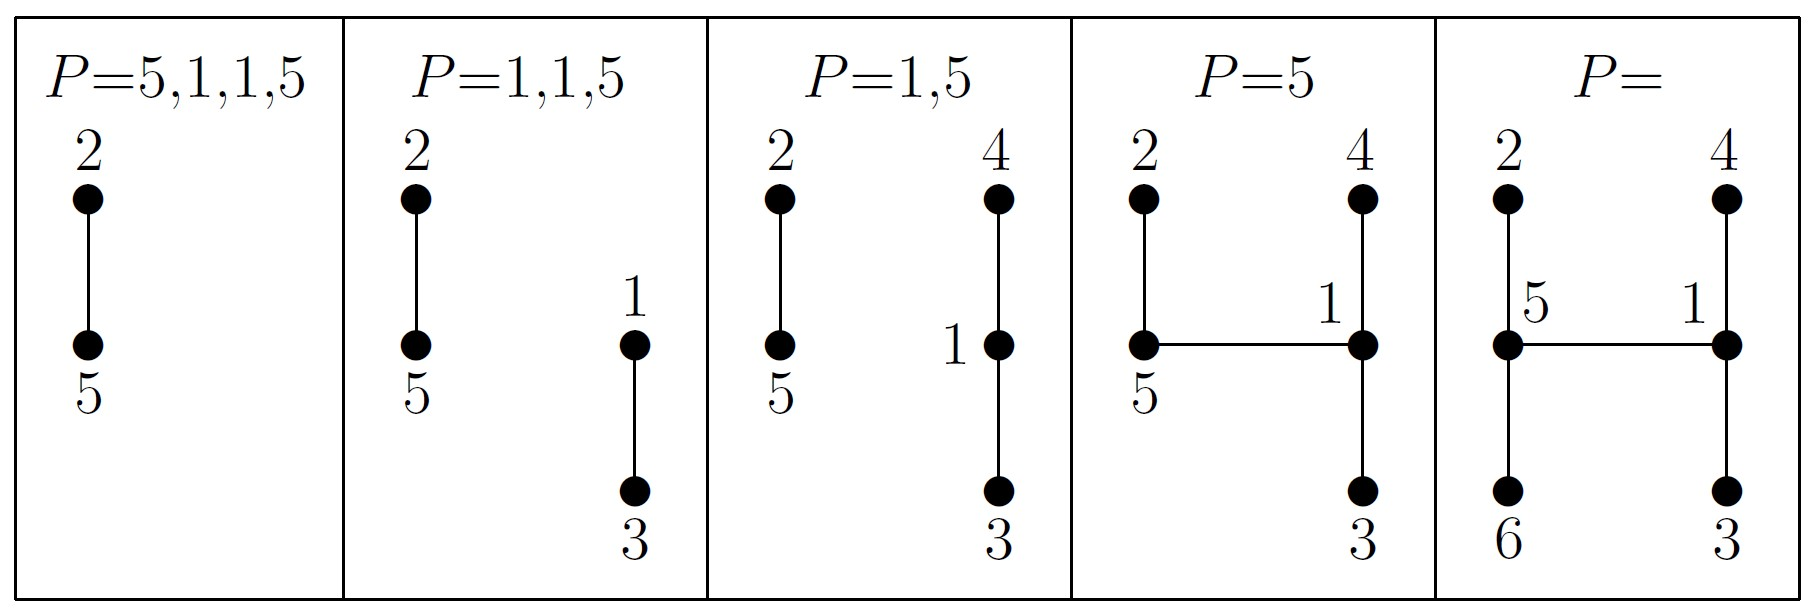
\includegraphics[width=9cm]{imatges/prufer2.jpg}
   \caption{A partir de la seqüència $P=(5,1,1,5)$, considerem el menor nombre del conjunt $\{1,\ldots,6\}$ tal que no estigui en $P$. Clarament aquest és el 2. Per tant, unim el vèrtex 2 amb el vèrtex indexat pel primer element de $P$, és a dir, amb el vèrtex 5. A continuació, eliminem el terme 5 de la seqüència $P$ i considerem la nova seqüència $P:=(1,1,5)$. Repetim el procés fins obtenir un seqüència $P$ buida. Finalment, cal unir el vèrtex 6 amb l'últim element de la seqüència $P$ inicial, és a dir, amb el vèrtex 5. \cite{3}}
   \label{pruf2}
\end{figure}
Podem veure, doncs, que per a cada arbre hi ha un única seqüència de Prüfer associada, i per a cada seqüència de Prüfer hi ha un únic arbre associat. El següent teorema (que ja queda demostrat amb els comentaris fets anteriorment) ens ho afirma formalment.
\begin{theorem}\label{bij}
Sigui $T_n$ el conjunt d'arbres generadors d'ordre $n$ i $\mathcal{P}_n$ el conjunt de seqüències de Prüfer de $n-2$ termes. Considerem la següent aplicació de conjunts:
\begin{align*}
    \varphi:T_n&\rightarrow \mathcal{P}_n\\
    T&\mapsto \mathcal{P}(T)
\end{align*}
Aleshores, $\varphi$ és bijectiva.
\end{theorem}
Ara sí, doncs, podem enunciar el teorema de Cayley:
\begin{theorem}[Teorema de Cayley]
Sigui $G=K_n$ un graf complet d'ordre $n\geq 2$.\footnote{Els casos trivials $n=1$ i $n=2$ no cal considerar-los.} Aleshores hi ha $n^{n-2}$ arbres generadors diferents.
\end{theorem}
\begin{proof}
El cas $n=2$ és immediat. Vegem el cas $n\geq3$.\par
Pel teorema \ref{bij} sabem que el nombre de seqüència de Prüfer està en bijecció amb el nombre d'arbres generadors d'ordre $n$, per tant tindrem que $\tau(G):=|T_n|=|\mathcal{P}_n|$. Ara bé, el conjunt $\mathcal{P}_n$ està format per paraules de longitud $n-2$ de l'alfabet $[n]$. Per tant, sabem que hi haurà $n^{n-2}$ paraules diferents i, per tant, tindrem que $\tau(G)=n^{n-2}$, tal com volíem demostrar.
\end{proof}
Vegem ara un exemple d'aplicació de la fórmula de Cayley:
\begin{example}\label{ex1}
Considerem el graf complet $K_4$, és a dir, el graf de la figura \ref{k4}.\par Per la fórmula de Cayley, el nombre d'arbres generadors és $4^{4-2} = 16$. A la figura \ref{k4_16} els podem veure tots.
\begin{figure}[H]
\centering
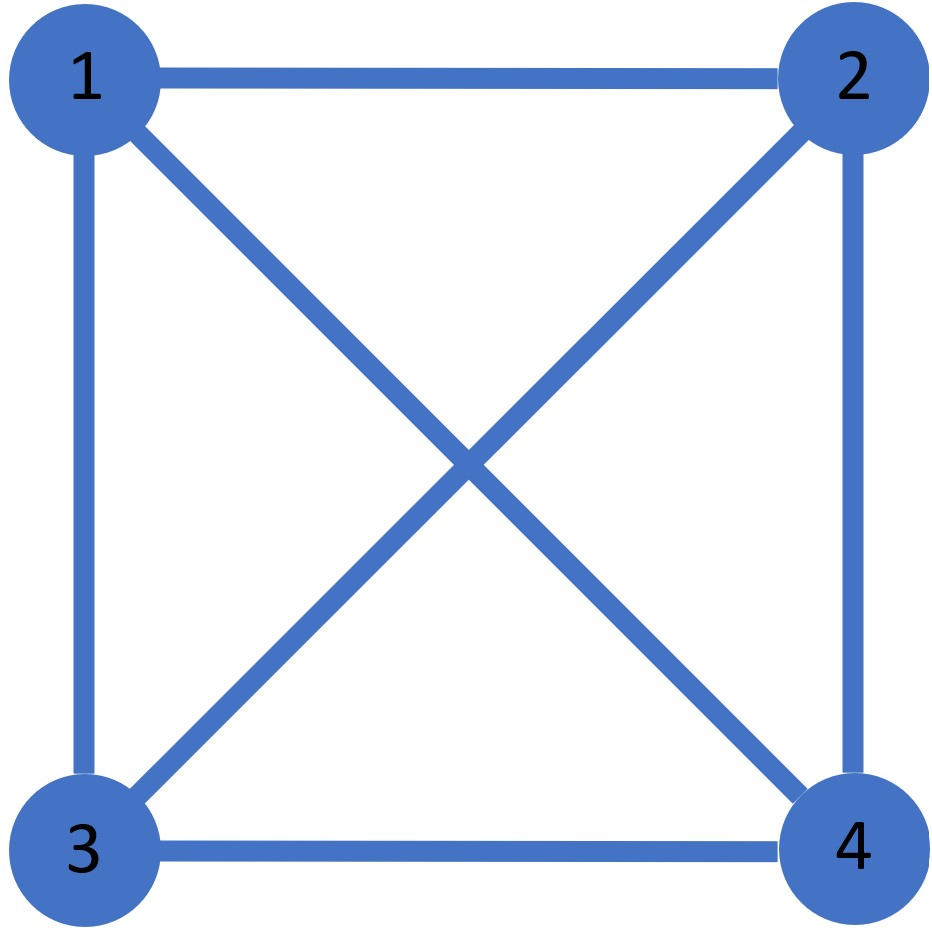
\includegraphics[width=4cm]{imatges/graf2.jpg}
  \caption{Graf $K_4$.}
  \label{k4}
\end{figure}
\begin{figure}[H]
\centering
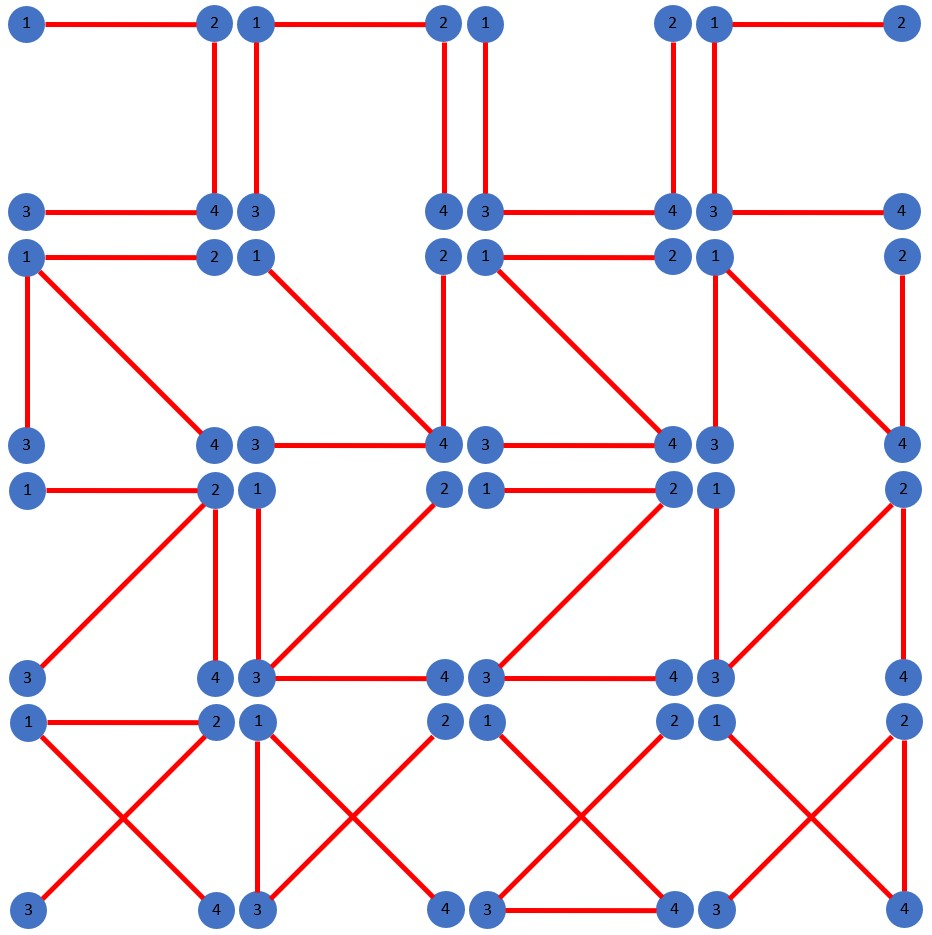
\includegraphics[width=9cm]{imatges/graf2_16.jpg}
  \caption{Arbres generadors diferents del graf complet $K_4$.}
  \label{k4_16}
\end{figure}
\end{example}
\begin{definition}
Donat un graf connex $G =(V,E)$ i $e = uv \in E(G)$, denotarem per $G_e$ el graf resultant de suprimir l'aresta $e$ del graf $G$ i identificar els vèrtexs $u$ i $v$ com a iguals.
\end{definition}
Un exemple de la creació d'aquest graf $G_e$ a partir d'un graf $G$, el podem trobar a la figura \ref{ge}.
\begin{figure}[H]
    \centering
    \begin{subfigure}{.45\textwidth}
        \centering
        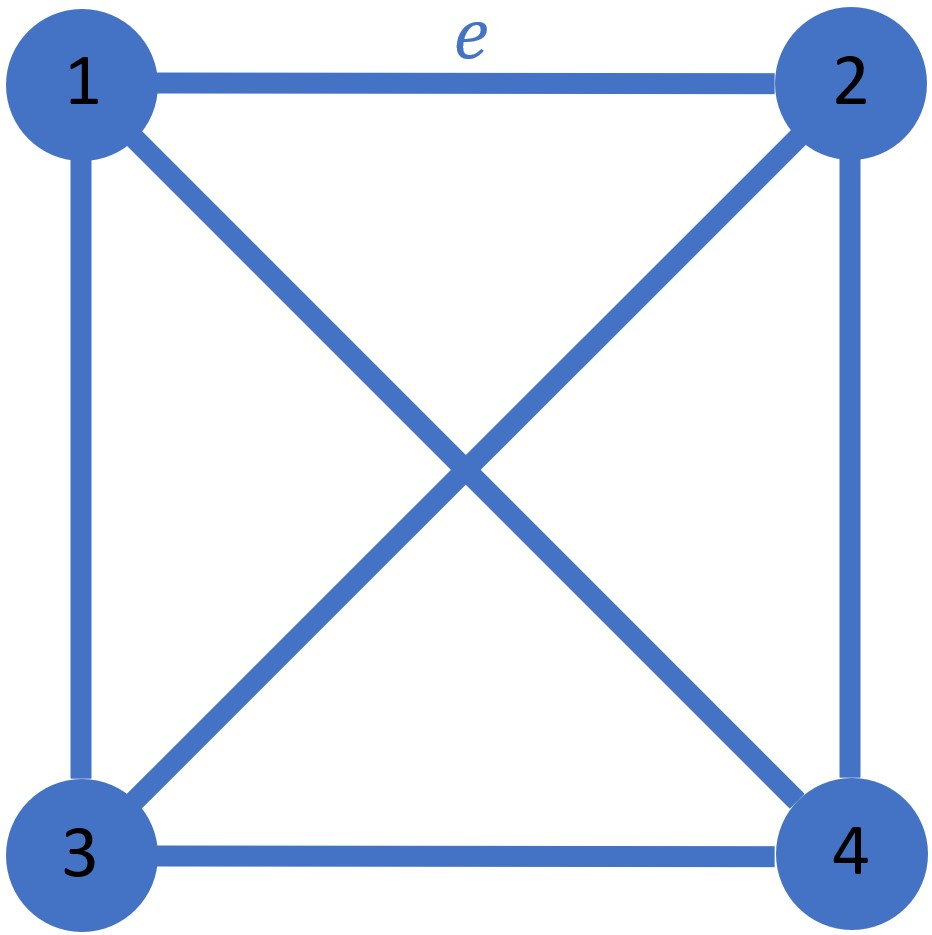
\includegraphics[width=3cm]{imatges/graf_e.jpg}
    \end{subfigure}
    \begin{subfigure}{.45\textwidth}
        \centering
        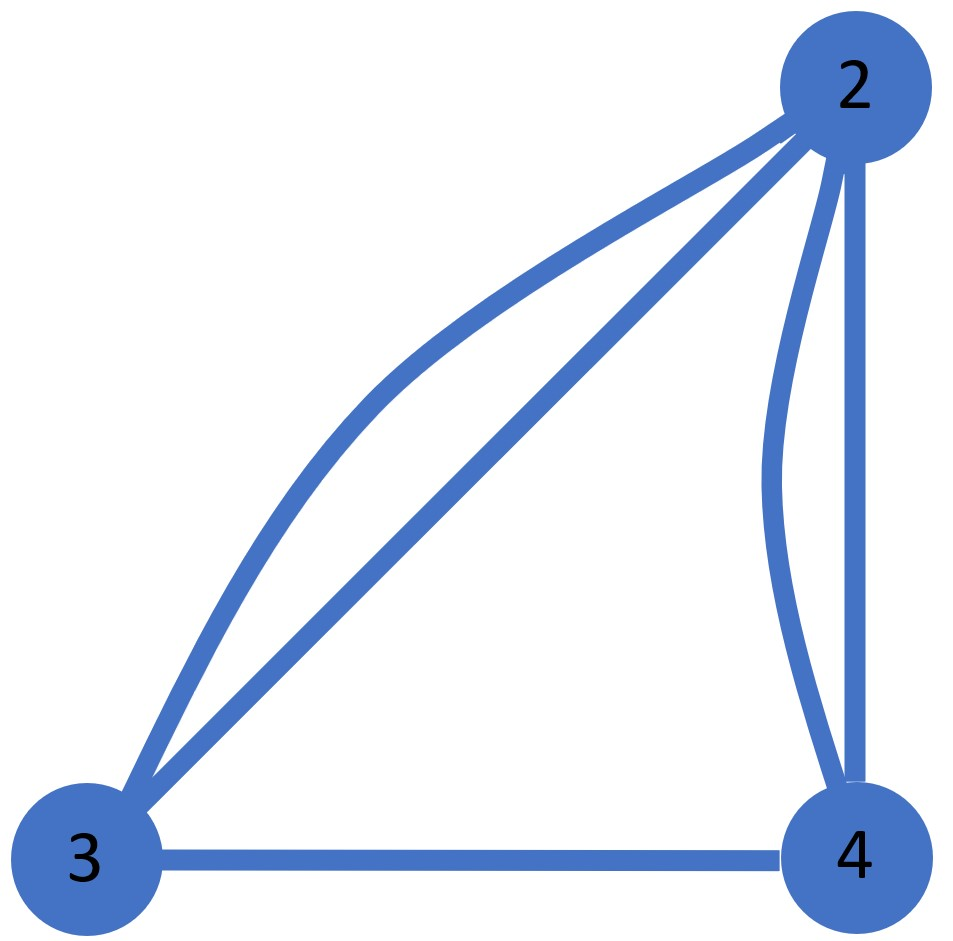
\includegraphics[width=3cm]{imatges/graf_e_reduit.jpg}
    \end{subfigure}
    \caption{A l'esquerra observem el graf $G=K_4$, amb l'aresta $e$ a suprimir. A la dreta hem creat el graf $G_e$, resultat de suprimir l'aresta $e$ i d'identificar els vèrtexs 1 i 2 en un de sol.}
    \label{ge}
\end{figure}
Vegem ara com el nombre $\tau(G)$ d'arbres generadors d'un graf $G$ (no simple) verifica el següent resultat:
\begin{theorem}
Sigui $G$ un multigraf. Donada $e\in E(G)$ una aresta de $G$, es compleix $$\tau(G)=\tau(G-e)+\tau(G_e).$$
\end{theorem}
\begin{proof}
Sigui $\tau(G)=\tau_1(G)+\tau_2(G)$, on $\tau_1(G)$ és el nombre d'arbres generadors de $G$ que no contenen l'aresta $e$ i $\tau_2(G)$ és el nombre d'arbres generadors de $G$ que contenen l'aresta $e$. És clar que la suma d'ambdós nombres dona $\tau (G)$. Observem, a més, que $\tau_1(G)=\tau(G-e)$ i $\tau_2(G)=\tau(G_e)$. \cite{1}
\end{proof}
\section{Nombre d'arbres generadors}
    L'objectiu ara és generalitzar la fórmula de Cayley i calcular el nombre d'arbres generadors que tenim en un graf $G$ connex arbitrari. Per això, necessitem uns resultats previs.
    \begin{lemma}\label{1}
    Sigui $G$ un graf connex d'ordre $n$. Si $M$ és la matriu d'incidència orientada de $G$ i $L$ és la matriu de Laplace de $G$, tenim que $$L=MM^t.$$
    \end{lemma}
    \begin{proof}
    Sigui $m=|E(G)|$ i $v_i,v_j\in V(G)$. Aleshores tenim que $$(MM^t)_{ij}=\sum_{k=1}^mM_{ik}M_{kj}^t=\sum_{e_k\in E(G)}M_{ik}M_{kj}^t=\sum_{e_k\in E(G)}M_{ik}M_{jk}.$$
    Distingirem dos casos: si $i\ne j$ o si $i=j$. Pel que fa al primer cas, tindrem que $M_{ik}M_{jk}\ne 0$ si i només si l'aresta $e_k$ connecta els vèrtexs $v_i$ i $v_j$. Ara bé, com que per definició de la matriu d'incidència orientada cada columna té un 1 o un $-1$, aleshores un els valors $M_{ik}$ i $M_{jk}$ serà 1 i l'altre serà $-1$ i, per tant, tindrem sempre que $M_{ik}M_{jk}=-1$. Repetint aquest procés per a tots els $k$ tals que $v_i$ i $v_j$ són incidents amb $e_k$ tindrem que $$(MM^t)_{ij}=\sum_{e_k\in E(G)}M_{ik}M_{jk}=-m_{ij},$$ on $m_{ij}$ és el nombre d'arestes que uneixen $v_i$ i $v_j$, tal com volíem veure.\par
    Pel que fa al cas $i=j$, tindrem que $M_{ik}M_{jk}=M_{ik}^2$ serà $(\pm 1)^2=1$ si $e_k$ és incident amb $v_i$ i 0 altrament. Per tant, fent la suma per $e_k\in E(G)$ tindrem que $(MM^t)_{ii}=\deg v_i$, com volíem demostrar. \cite{2}
    \end{proof}
    \begin{theorem}\label{2}
    Sigui $G$ un graf i $T$ un subgraf de $G$. Aleshores, $T$ és un arbre generador de $G$ si i només si $|\det M_0[T]|=1$.
    \end{theorem}
    \begin{proof}
    Sigui $n=|V(G)|$. Considerarem els tres possibles casos per a un subgraf $H$ de $G$: $H$ que sigui un arbre generador de $G$; $H$ que sigui un subgraf generador de $G$ no connex amb $n-1$ arestes, o $H$ que no sigui un subgraf generador.\par
    Sigui $T=H$ un arbre generador de $G$, $v_r$ el vèrtex de referència de $M_0$ i $u_1\ne v_r$ una fulla de $T$. Denotem $e_1$ l'aresta de $T$ incident amb $u_1$. Més en general, sigui $u_i\ne v_r$, $i=1,2,\ldots, n-1$, una fulla de l'arbre $T-\{u_1,\ldots,u_{i-1}\}$ i $e_i$ l'aresta incident amb $u_i$ en aquest arbre. Observem que ara, permutant adequadament les files de $M_0[T]$, podem obtenir una matriu $M_0[T]'$ tal que 
    $$
    |(M_0[T]')_{ij}|=\left\{\begin{array}{ll}
        1 & \text{si $u_i$ és incident amb $e_j$,} \\
        0 & \text{altrament.}
    \end{array}\right.$$
    Així doncs, per construcció, $M_0[T]'$ és de la forma
    $$M_0[T]'=\begin{pmatrix}
    1 & 0 & \cdots & 0\\
    * & 1 & \ddots & \vdots \\
    \vdots & \ddots & \ddots & 0\\
    * & \cdots & * & 1
    \end{pmatrix}.$$
    Com que $M_0[T]'$ és una matriu triangular inferior i permutacions en les columnes no alteren el valor absolut del determinant, tenim que $|\det M_0[T]|=|\det M_0[T]'|=1$.\par
    En canvi, si $H$ és un subgraf generador de $G$ no connex amb $n-1$ arestes, la suma de les files de $M_0[H]$ corresponents als vèrtexs de $H$ que no siguin adjacents al vèrtex $v_r$ dona el vector 0 ja que en cada columna sumem 1 i $-1$. Per tant, fent aquesta combinació de files (que no altera el valor del determinant, llevat del signe) tenim que $\det M_0[H]=0$.\par
    Finalment, si $H$ no és subgraf generador de $G$ i no conté $v_r$, aleshores la suma de totes les columnes de $M_0[H]$ dona, seguint el mateix raonament d'abans, el vector 0. Si $H$ no és subgraf generador de $G$ i conté $v_r$, aleshores existeix un vèrtex $v_i\in V(G)\setminus V(H)$. En particular la fila $i$-èssima de $M_0[H]$ serà el vector 0. En qualsevol dels dos casos tindrem que $\det M_0[H]=0$. \cite{1}
    \end{proof}
    Per demostrar el teorema que ens dirà el nombre d'arbres generadors d'un graf, necessitarem utilitzar la fórmula de Cauchy-Binet per al càlcul de determinants que recordem (i no demostrem) a continuació:
    \begin{theorem}[Fórmula de Cauchy-Binet]
    Sigui $A\in\mathcal{M}_{n\times m}(\mathbb{R})$ i $B\in\mathcal{M}_{m\times n}(\mathbb{R})$. Donat qualsevol subconjunt $S\subset\{1,\ldots,m\}$ tal que $|S|=n$, formem la matriu $A_S\in\mathcal{M}_n(\mathbb{R})$ escollint les columnes de $A$ indexades pel conjunt $S$ i formem la matriu $B_S\in\mathcal{M}_n(\mathbb{R})$ escollint les files de $B$ indexades pel conjunt $S$. Aleshores tenim que $$\det(AB)=\sum_S\det(A_S)\det(B_S).$$
    \end{theorem}
    Passem ara a enunciar el nombre d'arbres generadors d'un graf.
    \begin{theorem}[Teorema de Kirchhoff]
    Sigui $G$ un graf connex amb matriu de Laplace $L$. Sigui $n=|V(G)|$, $m=|E(G)|$ i sigui $L_i$ la matriu resultant d'haver tret a $L$ la fila i columna $i$-èssimes, per a qualsevol $i\in\{1,\ldots,n\}$. Aleshores, el valor $\det L_i$ és independent de $i$ i el nombre $\tau(G)$ d'arbres generadors de $G$ és $$\tau(G)=\det L_i.$$
    \end{theorem}
    \begin{proof}
    Com que $M_0$ l'hem creada suprimint l'última fila de $M$ ho demostrarem únicament per $L_0:=L_n$. Com que, pel lema \ref{1}, tenim que $L=MM^t$, és clar que tindrem $L_0=M_0M_0^t$.
    Per la fórmula de Cauchy-Binet aplicat a les matrius $M_0$ i $M_0^t$ tenim que \begin{equation}
        \det L_0=\det(M_0M_0^t)=\sum_S\det((M_0)_S)\det((M_0^t)_S),
        \label{eq1}
    \end{equation} on $S\subset\{1,\ldots,m\}$ tal que $|S|=n$. Ara bé, en general tenim que per una matriu $A\in\mathcal{M}_{p\times q}(\mathbb{R})$ es compleix $(A^t)_S=(A_S)^t$, i aleshores l'equació \ref{eq1} esdevé 
    \begin{equation}
        \det L_0=\sum_S(\det(M_0)_S)^2.
        \label{eq2}
    \end{equation}
    Ara bé, pel teorema \ref{2} tenim que $(\det(M_0)_S)^2=1$ si les arestes indexades per $S$ defineixen un arbre generador de $G$ y $(\det((M_0)_S))^2=0$, en cas contrari. Per tant, és clar que que la suma de l'equació \ref{eq2} compta el nombre total d'arbres generadors, és a dir, $\tau(G)=\det L_0$. \cite{2}
    \end{proof}
    L'objectiu ara és trobar algun mètode alternatiu per al càlcul de $\tau(G)$. Abans de seguir, però, necessitarem aquest resultat d'àlgebra lineal:
    \begin{lemma}\label{3}
    Sigui $A\in\mathcal{M}_n(\mathbb{R})=(a_{ij})$ tal que $\displaystyle\sum_{i=1}^na_{ij}=\sum_{j=1}^na_{ij}=0$ per a tot $i,j\in[1,n]$, és a dir, la suma de tots els elements de cada fila i columna és nul·la. Sigui $A_0$ la matriu obtinguda de $A$ eliminant la fila i columna $i$-èssimes, per a qualsevol $i\in[1,n]$. Aleshores, el coeficient de $x$ del polinomi característic de $A$ és $-n\cdot\det A_0$. A més el terme constant de $\det(A-xI)$ és 0.
    \end{lemma}
    \begin{proof}
    El terme constant de $\det(A-xI)$ és $\det A$, que és 0 ja que totes les files sumen 0 i, per tant, els vectors de les files de $A$ són linealment dependents. Això explica que $A$ tingui, com a mínim, un valor propi igual a 0.\par
    Pel que fa a l'altra afirmació del lema, suposarem (sense pèrdua de generalitat) que hem creat $A_0$ eliminant l'última fila i columna de $A$. Tenim doncs que:
    \begin{multline*}
    \det(A-xI)=\begin{vmatrix}
    a_{11}-x & a_{12} & \cdots & a_{1n}\\
    a_{21} & a_{22}-x & \ddots & \vdots\\
    \vdots & \ddots & \ddots & a_{(n-1)n}\\
    a_{n1} & \cdots & a_{n(n-1)} & a_{nn}-x\\
    \end{vmatrix}=\left|\begin{array}{@{\,} ccc|c @{\,}}
    & & & a_{1n}\\
    & A_0(x) & & \vdots\\
    & & & a_{(n-1)n}\\
    \hline
    a_{n1} & \cdots & a_{n(n-1)} & a_{nn}-x\\
\end{array}\right|=\\=\left|\begin{array}{@{\,} ccc|c @{\,}}
    & & & a_{1n}\\
    & A_0(x) & & \vdots\\
    & & & a_{(n-1)n}\\
    \hline
    -x & \cdots & -x & -x\\
\end{array}\right|=-x\left|\begin{array}{@{\,} ccc|c @{\,}}
    & & & a_{1n}\\
    & A_0(x) & & \vdots\\
    & & & a_{(n-1)n}\\
    \hline
    1 & \cdots & 1 & 1\\
\end{array}\right|.
    \end{multline*}
    Aquí per simplificar la notació hem definit la matriu $A_0(x)$, hem sumat totes les files (excepte l'última) a l'última i hem tingut en compte la hipòtesi inicial de la suma dels elements de les columnes de $A$. Reduïm, doncs, el problema a calcular el terme independent del polinomi $$\left|\begin{array}{@{\,} ccc|c @{\,}}
    & & & a_{1n}\\
    & A_0(x) & & \vdots\\
    & & & a_{(n-1)n}\\
    \hline
    1 & \cdots & 1 & 1\\
\end{array}\right|.$$
    Ara bé, fent $x=0$ i sumant totes les columnes (excepte l'última) a l'última tenim que: $$\left|\begin{array}{@{\,} ccc|c @{\,}}
    & & & a_{1n}\\
    & A_0(0) & & \vdots\\
    & & & a_{(n-1)n}\\
    \hline
    1 & \cdots & 1 & 1\\
\end{array}\right|=\left|\begin{array}{@{\,} ccc|c @{\,}}
    & & & 0\\
    & A_0 & & \vdots\\
    & & & 0\\
    \hline
    1 & \cdots & 1 & n\\
\end{array}\right|=n\det A_0,$$
    on hem utilitzat de nou la hipòtesi de l'enunciat i hem desenvolupat el determinant per l'última columna. Això acaba la demostració. \cite{2}
    \end{proof}
    \begin{corollary}\label{cor1}
    Sigui $G$ un graf connex tal que $n=|V(G)|$. Suposem que els valors propis de $L$ són $\lambda_1,\ldots,\lambda_n$, amb $\lambda_n=0$. Aleshores, $$\tau(G)=\frac{1}{n}\lambda_1\lambda_2\ldots\lambda_{n-1}.$$ 
    \end{corollary}
    \begin{proof}
    Notem que a la demostració anterior hem observat que sempre hi ha, com a mínim, un valor propi igual a 0. Per tant, té sentit considerar $\lambda_n=0$.\par
    Desenvolupant el polinomi característic $p_L(x)$ de $L$ tenim que: $$p_L(x)=\det(L-xI)=\prod_{i=1}^n(\lambda_i-x)=-x\prod_{i=1}^{n-1}(\lambda_i-x).$$ Per tant, el coeficient de $x$ en $p_L(x)$ és $-\lambda_1\lambda_2\ldots\lambda_{n-1}$. D'altra banda, pel lema \ref{3} tenim que el coeficient de $x$ és $-n\det L_0$, és a dir, $$-\lambda_1\lambda_2\ldots\lambda_{n-1}=-n\det L_0=-n\tau(G),$$ pel teorema de Kirchhoff. I finalment $$\tau(G)=\frac{1}{n}\lambda_1\lambda_2\ldots\lambda_{n-1}.$$ \cite{2}
    \end{proof}
    \begin{example}
       Considerem el graf $G$ de la figura \ref{graf1}.
       \begin{figure}[H]
           \centering
           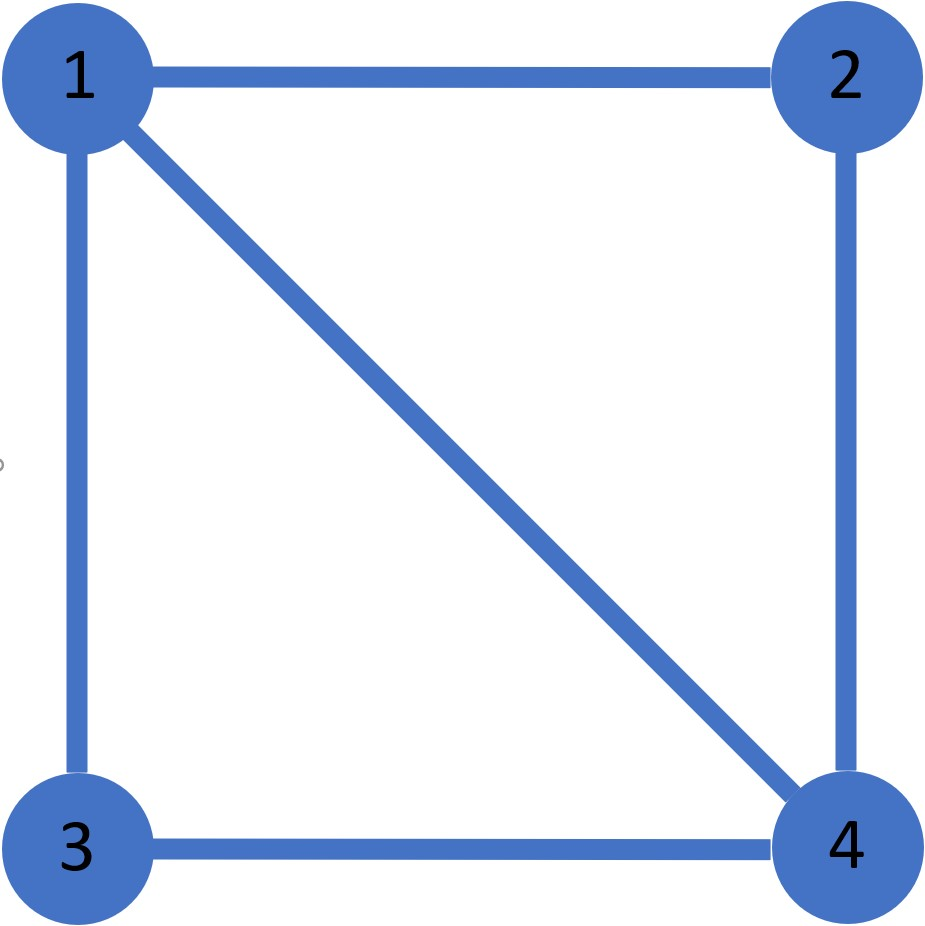
\includegraphics[width=4cm]{imatges/graf1.jpg}
           \captionof{figure}{}
           \label{graf1}
       \end{figure}
       Volem calcular el nombre d'arbres generadors d'aquest graf. Per això necessitem trobar la matriu de Laplace associada. En aquest cas tenim que $$L=\begin{pmatrix}
       3 & -1 & -1 & -1\\
       -1 & 2 & 0 & -1\\
       -1 & 0 & 2 & -1\\
       -1 & -1 & -1 & 3\\
       \end{pmatrix}.$$
       Calcularem el valor de $\tau(G)$ mitjançant els dos mètodes que hem exposat.
       \begin{enumerate}
           \item Utilitzant el teorema de Kirchhoff, podem crear $L_0$ suprimint la primera fila i columna de $L$. Així tenim que $$\tau(G)=\det L_0=\begin{vmatrix}
            2 & 0 & -1\\
            0 & 2 & -1\\
            -1 & -1 & 3\\
            \end{vmatrix}=8.$$
            \item Utilitzant el mètode del corol·lari \ref{cor1} hem de calcular el polinomi característic de $L$. Tenim doncs que:
            \begin{multline*}
                \det(L-xI)=\begin{vmatrix}
        3-x & -1 & -1 & -1\\
       -1 & 2-x & 0 & -1\\
       -1 & 0 & 2-x & -1\\
       -1 & -1 & -1 & 3-x\\
    \end{vmatrix}=\begin{vmatrix}
        -x & -1 & -1 & -1\\
       -x & 2-x & 0 & -1\\
       -x & 0 & 2-x & -1\\
       -x & -1 & -1 & 3-x\\
    \end{vmatrix}=\\=-x\begin{vmatrix}
        1 & -1 & -1 & -1\\
        1 & 2-x & 0 & -1\\
        1 & 0 & 2-x & -1\\
        1 & -1 & -1 & 3-x\\
    \end{vmatrix}=-x\begin{vmatrix}
        1 & 0 & 0 & 0\\
        1 & 3-x & 1 & 0\\
        1 & 1 & 3-x & 0\\
        1 & 0 & 0 & 4-x\\
    \end{vmatrix}=-x(4-x)[(3-x)^2-1]=x(x-2)(x-4)^2.
            \end{multline*}
            Per tant, els valors propis de $L$ són $\lambda_1=2$, $\lambda_2=\lambda_3=4$ i $\lambda_4=0$. Finalment, tenim que $$\tau(G)=\frac{1}{4}\lambda_1\lambda_2\lambda_3=8,$$ com era d'esperar.
       \end{enumerate}
       En la figura \ref{graf1_8} observem els 8 arbres generadors del graf $G$. Observem que el graf considerat en aquest exemple és un subgraf del graf $K_4$ i, evidentment, tots els seus arbres generadors són arbres generadors del graf $K_4$ (estudiat en l'exemple \ref{ex1}).
       \begin{figure}[H]
           \centering
           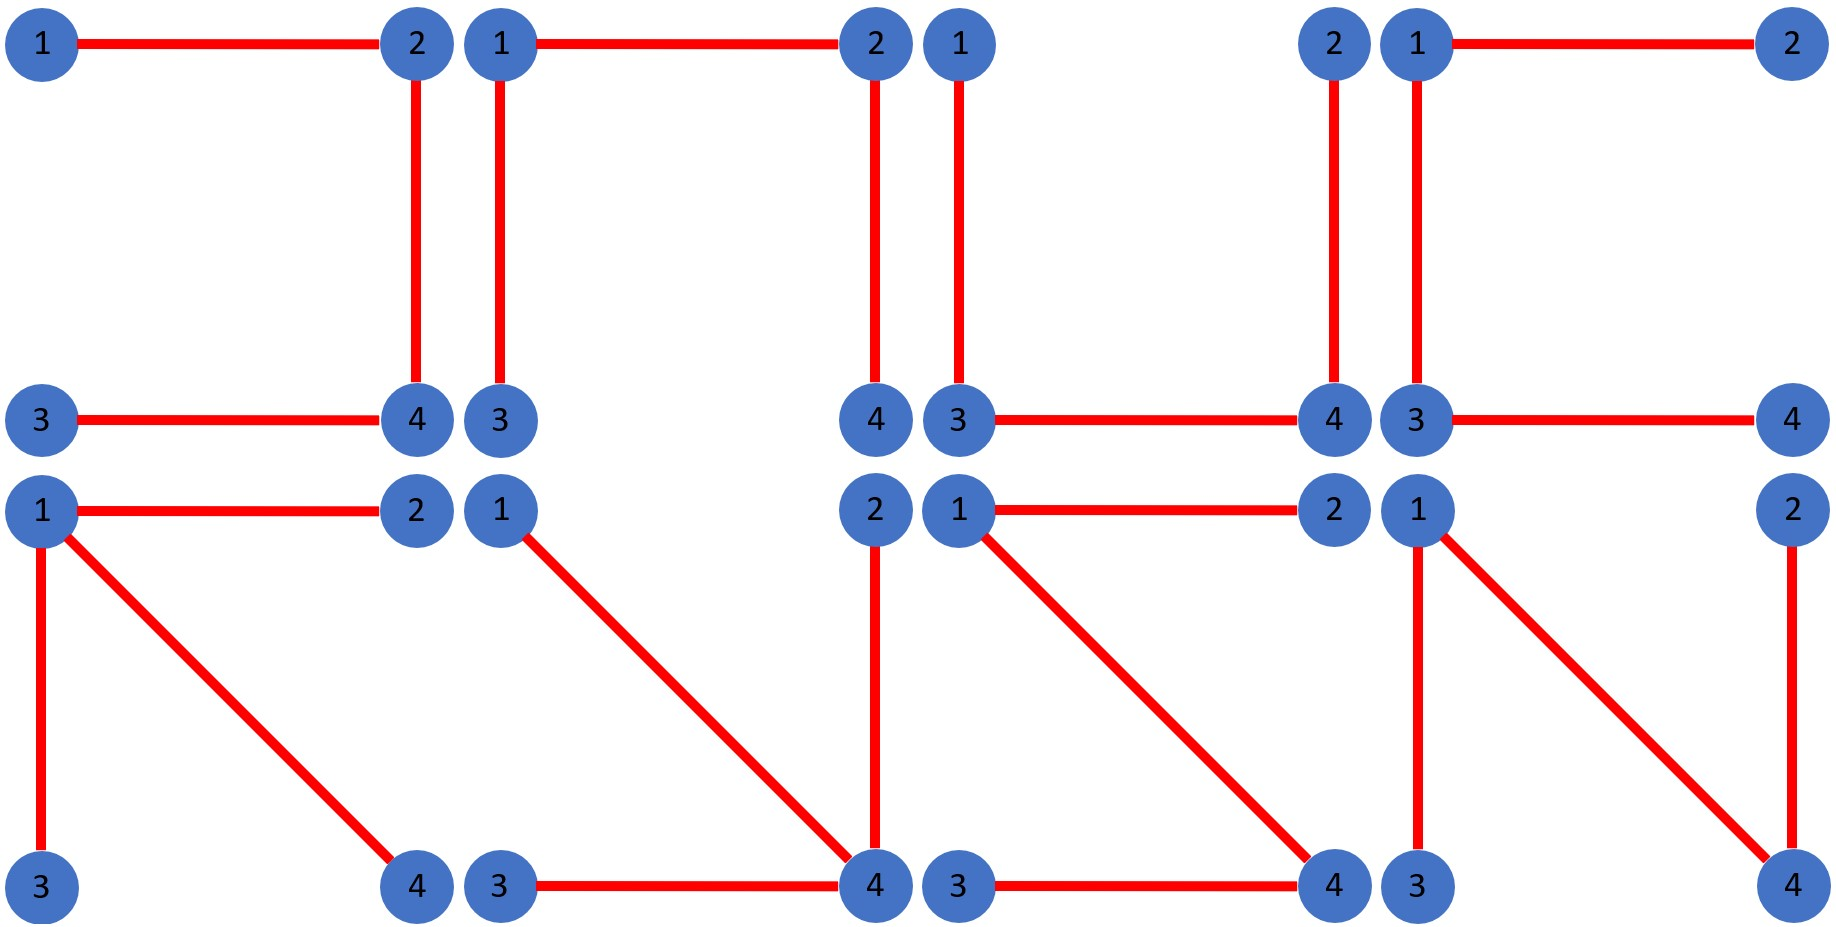
\includegraphics[width=9cm]{imatges/graf1_8.jpg}
           \captionof{figure}{}
           \label{graf1_8}
       \end{figure}
    \end{example}
\section{Aplicacions}
Abans de presentar les aplicacions referents als arbres generadors, necessitem definir uns quants conceptes.
\begin{definition}
Donat un graf $G$, diem que aquest és un graf ponderat, pesat o amb costos quan les arestes tenen associades un valor, és a dir, per a tot $e\in E(G)$ considerem el cost $w(e)$ associat a l'aresta $e$.
\end{definition} 
En introduir aquest nou element (els pesos) se'ns obre una gran varietat d’aplicacions dels grafs, principalment en l’àmbit de l’optimització. Entre d'altres, algunes són:
\begin{itemize}
    \item Arbres generadors de diàmetre mínim amb pesos
    \item Arbres generadors de camins mínims
    \item Arbres generadors més i menys uniformes
    \item Arbre mínim d’Steiner
    \item Arbres generadors de cost mínim
\end{itemize}
En aquest treball ens centrem a desenvolupar més en profunditat els arbres generadors de cost mínim, treballant amb grafs connexos i no dirigits.\footnote{Un graf dirigit és un tipus de graf en el qual les arestes tenen un sentit definit, és a dir, estan orientades d'un vèrtex cap a l'altre.}\par

Determinar quin és l’arbre generador de cost mínim ens permetrà, per exemple, saber la ruta més curta per anar d’una ciutat a una altra (aquests són una part important dels càlculs que fan els navegadors GPS) o resoldre problemes dins l’àmbit de les xarxes de comunicació, les xarxes elèctriques i la telefonia on els vèrtexs representarien punts de consum elèctric, telèfons, aeroports o computadores, i les arestes serien els cables d’alta tensió, de fibra òptica o les rutes aèries.
\begin{definition}
Donat un graf $G$ ponderat per una funció $w(e)$ i un arbre generador $T$ de $G$ definim el pes de l’arbre $T$ com $$w(T)=\sum_{e\in E(G)} w(e).$$
\end{definition} 
\begin{definition}
Un arbre generador minimal, o de cost mínim, de $G$ és un arbre generador $T$ de $G$ de pes $w(T)$ mínim.
\end{definition}
Per tal de determinar l’arbre generador de cost mínim d’un graf, farem ús de diferents algoritmes en funció de les característiques del graf.\par La nostra intuïció ens condueix al que s'anomena ``algoritme de força bruta", que consisteix a trobar tots els arbres generadors i fer comparacions entre ells per tal de determinar-ne el de pes mínim. Tal com podem intuir, no és gens eficient. A continuació, exposem de manera detallada dos algoritmes per grafs connexos, no dirigits i ponderats d’ordre $n$ i mida $m$.
\subsection{Algoritme de Prim}
L'algoritme de Prim va ser dissenyat per primer cop el 1930 pel matemàtic Vojtech Jarnik i més endavant, de manera independent, pel científic Robert C. Prim en 1957. \cite{12}\par
La idea bàsica de l'algoritme de Prim per determinar l'arbre generador de cost minimal és començar escollint un vèrtex $v\in V(G)$ qualsevol i considerar tots els vèrtexs $u_i$ adjacents a $v$ a través de l'aresta $e_i^1$, $i=1,\ldots,r$. Agafem doncs l'aresta $e_k^1$ que tingui el cost mínim. Ara considerem els vèrtexs $u_k,v$ i considerem tots els vèrtexs $p_j$ adjacents a $u_k$ i $v$ a través de l'aresta $e_j^2$, $j=1,\ldots,s$. Agafem, doncs, $e_k^2$ que tingui un cost mínim. Repetint aquest pas fins que tinguem $n-1$ arestes, obtindrem l’arbre generador minimal.
\begin{prop}[Algoritme de Prim]
Sigui $G$ un graf. Per crear l'arbre generador de cost mínim seguim els següents passos:
\begin{enumerate}
    \item Escollim un vèrtex $v_1\in V(G)$ i considerem l’arbre $T$ format pel vèrtex $v_1$.
    \item Sigui $e'$ l’aresta de pes mínim incident a un vèrtex de $T$ i un altre vèrtex $u\notin V(T)$. A continuació, creem el nou arbre $T:=T+e'$.
    \item Si $|E(T)|=n-1$ ja hem acabat. Si no, tornem al pas 2.
\end{enumerate}
\end{prop}
L’elecció del vèrtex inicial pot fer que l’arbre generat sigui diferent, però en qualsevol cas serà de cost mínim.\par A continuació, exposarem el pseudocodi de l'algoritme de Prim.
\subsubsection{Pseudocodi de l'algoritme de Prim}
Les estructures necessàries per a la implementació de l'algoritme són les següents:
\begin{itemize}
    \item Un graf connex $G$ i ponderat amb una funció $w(e)$ que assigna un pes a cada aresta.
    \item Un conjunt $U$ dels vèrtexs que ja s'han visitat.
    \item Una etiqueta $(E(u),v_i)$ a cada vèrtex $u$ que registra el pes ($E(u)$) de l'aresta de pes mínim que connecta el vèrtex $u$ amb un vèrtex $v_i$ ja visitat. Al final, la taula $(E(v_i),\cdot)$, $i=1,\ldots,n$ enregistra els pesos de les arestes que formen part de l'arbre generador minimal.
\end{itemize}
Com hem explicat anteriorment, en cada pas es fixa l'etiqueta d'un dels vèrtexs del graf. D'aquesta manera, després de $n$ passos haurem calculat l'arbre generador minimal. El pseudocodi és el següent: 
\begin{algorithm}[H]
\caption{\textbf{- Algoritme de Prim}}
\begin{algorithmic}
\item \algorithmicrequire{Graf ponderat $(G,w)$ connex d’ordre $n$.}
\item \algorithmicensure{Arbre generador minimal T.}
\State 
\State Seleccionem un vèrtex aleatori inicial $u_0\in V(G)$;
\State $\text{U}:=\emptyset$;
\For{$v\in V\setminus\{u_0\}$}
\State $\text{E}(v):=\infty$;  //valor per defecte per si no existeix l'aresta que uneix un element de $U$ amb un de $V$
\State Etiquetem $v$ amb $(E(v),u_0)$;
\EndFor
\State $E(u_0):=0$;
\State Etiquetem ${u_0}$ amb (0,${u_0}$);
\State $A:=\emptyset$;
\For {$i=1$ \textbf{to} $n$}
\State $E(u_i):=\min\{E(v): v\in V\setminus U\}$;
\State $x:=\text{vèrtex de $U$ incident amb $u_i$}$;
\State$U\gets U\cup \{u_i\}$;
\State$A\gets A\cup \{xu_i\}$; //on $(E(u_i),x)$ es l'etiqueta de $u_i$
\For {$v\in V\setminus U: v\text{ adjacent a } u_i$}
\If {$w(u_iv) < E(v)$}
\State $E(v):=w(u_iv)$;
\State Etiquetem $v$ amb $(E(v),u_i)$;
\EndIf
\EndFor
\EndFor
\State $T \gets (V,A)$;
\State\Return $T$;
\end{algorithmic}
\end{algorithm}
\par\cite{7}\par 
L’algoritme de Prim té una complexitat de $O(n^2)$. En efecte, si $T$ és l'arbre que es va construint, cada iteració té una complexitat de $O(n)$ en buscar el vèrtex no pertanyent a $V(T)$ amb aresta incident de mínim cost i adjacent a un vèrtex de $V(T)$. Si tenim en compte que això es repeteix $n$ vegades, obtenim una complexitat total de $O(n^2)$. Notem, però, que si aquest algoritme s’implementa amb monticles\footnote{En aquest cas, entenem un monticle com un arbre en el qual les arestes estan ordenades pel seu pes.}, el temps requerit per l’algoritme és de $O(m\log n)$. \cite{6}
\subsection{Algoritme de Kruskal}
L'algoritme de Kruskal va ser escrit i publicat el 1956 per Joshep Kruskal. \cite{11}\par
La idea bàsica de l'algoritme de Kruskal és la següent: es tracta d'un algoritme voraç (\textit{Greedy algorithm}), que es caracteritzen per trobar una ``bona solució", que no vol dir que sigui la més òptima, en un interval de temps curt. L’estratègia és anar incorporant arestes de mínim pes fins aconseguir un arbre generador. Cada vegada que s’incorpora una aresta s’ha de comprovar que no forma cap cicle.
\begin{prop}[Algoritme de Kruskal]
Sigui $G$ un graf. La descripció de l'obtenció de l'arbre generador de cost mínim a través de l'algoritme de Kruskal és la següent:
\begin{enumerate}
    \item Escollim l'aresta de pes mínim $e$ i considerem l'arbre $T$ format per aquesta aresta.
    \item Sigui $e'$ l’aresta de pes mínim tal que $e'\notin E(T)$ i $T+e'$ no forma cap cicle. Aleshores, considerem el nou graf $T:=T+e$.
    \item Si $|E(T)|=n-1$ ja hem acabat. Si no, tornem al pas 2.
\end{enumerate}
\end{prop}
A continuació, exposem el pseudocodi de l'algoritme de Kruskal.
\subsubsection{Pseudocodi de l'algoritme de Kruskal}
Les estructures necessàries per a la implementació de l'algoritme són les següents: 
\begin{itemize}
    \item Un graf connex $G$ i ponderat amb una funció $w(e)$ que assigna un pes a cada aresta.
    \item Les funcions següents:
    \begin{itemize}
        \item $cerca (u)$: retorna el conjunt que conté el vèrtex $u$.
        \item $unio (u,v)$: realitza la unió dels conjunts $X$ i $Y$ que contenen els vèrtexs $u$ i $v$, respectivament, a través de l'aresta $uv$.
    \end{itemize}
\end{itemize}
El pseudocodi d'aquest algoritme és el següent: 
\begin{algorithm}[H]
\caption{\textbf{- Algoritme de Kruskal}}
\begin{algorithmic}
\item \algorithmicrequire{Graf ponderat $(G,w)$ connex d’ordre $n$.}
\item \algorithmicensure{Arbre generador minimal T.}
\State
\State Ordenem el conjunt de les arestes $E(G)$ segons $w(e)$ en ordre ascendent;
\State $A:=\emptyset$;
\For{$v\in V(G)$}
\State Creem el conjunt $\{v\}$;
\EndFor
\For {$uv\in E(G)$}
\If {$|A|=n-1$}
\State\textbf{break};
\EndIf
\State $X=cerca(u)$;
\State $Y=cerca(v)$;
\If {$X\ne Y$}
\State $A\gets A\cup \{uv\}$;
\State $unio(u,v)$;
\EndIf
\EndFor
\State $T\gets (V,A)$;
\State \Return $T$;
\end{algorithmic}
\end{algorithm}
\par \cite{7} \cite{8} 
\par
Parlem ara de la complexitat d'aquest algoritme. La primera part tracta d’ordenar la llista d’arestes en funció del seu pes. Mitjançant algoritmes com, per exemple, el \textit{quicksort} o \textit{heapsort} obtindrem una complexitat $O(m\log m)$, on $m$ és el nombre d’arestes. D'altra banda, les dues operacions de cerca que es fan en cada iteració es poden realitzar en un màxim de $O(\log m)$ passos. Tenint en compte que bucle s'executa un nombre proper a $n$ vegades, obtindríem una complexitat de $O(n\log m)$.
Tot l’algoritme tindrà una complexitat que vindrà donada per $\max\{O(m\log m),O(n\log m)\}$. Com que, per a un graf connex tenim que $m\geq n-1$, podem concloure que l’algoritme de Kruskal té una complexitat $O(m\log m)$.\par
Arribats en aquest punt, ens preguntem quin dels algoritmes és més eficient o quin convé utilitzar. La resposta és que depèn del nombre d’arestes del graf. Si el graf té un nombre proper al màxim d'arestes possibles, és a dir, el graf és ``proper" a ser un graf complet, tenim que $|E(G)|= O(n^2)$ ja que un graf complet té $n(n-1)/2$ arestes. Per tant, pel que fa a l’algoritme de Kruskal, trobem una complexitat de $O(n^2\log n)$ mentre que l’algoritme de Prim té una complexitat de $O(n^2)$ i, per tant, concloem que l’algoritme de Prim seria el més adequat.\par
En cas que el nombre d’arestes fos més proper al nombre de vèrtexs del graf, tindríem que $|E(G)|=O(n)$ i per tant l’algoritme de Kruskal tindria una complexitat de $O(n\log n)$, mentre que en el de Prim seria de $O(n^2)$. En aquest cas, doncs, convindria més utilitzar l’algoritme de Kruskal. \cite{6}

\newpage
\printbibliography[heading=bibintoc,title={Referències}]

\end{document}
